\section{Resultados}

\subsection{Datos de desarrollo (EEG\_1)}\label{sec:dev}

\paragraph{Mezclar segmentos de la misma persona explica la mayor parte de la exactitud reportada.} Con los 19 canales y LOSO por persona, la réplica obtuvo 49.9--56.6\,\% (exactitud de segmentos promediada por persona) en seis combinaciones representativas, cerca del 54\,\% que se obtiene prediciendo siempre la clase mayoritaria (Fig.~\ref{fig:dev}). Cuando se permitió que segmentos de la misma persona quedaran en entrenamiento y prueba (validación cruzada de 10 particiones por registro), las mismas características y clasificadores alcanzaron 89.8--99.2\,\%. El valor que \citet{aljalal2024} reportan para su mejor combinación con todos los canales (DWT-STD-LDA, 89.7\,\%) está más cerca de nuestra estimación por registro (89.8\,\%) que de la estimación por persona (54.4\,\%).

\begin{figure}[t]
\centering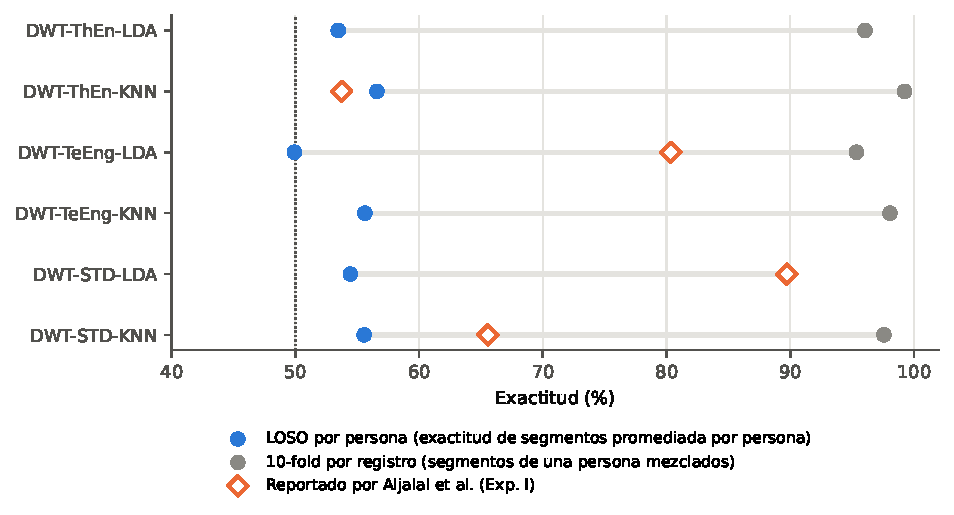
\includegraphics[width=\linewidth]{../figs/es_dev.pdf}
\caption{\textbf{Validación por persona frente a validación por registro en los datos de desarrollo.} Mismas características DWT y clasificadores, 19 canales, EEG\_1 (24 personas). Azul: LOSO, excluyendo del entrenamiento todos los segmentos de la persona evaluada. Gris: validación de 10 particiones sobre segmentos, que mezcla segmentos de la misma persona. Rombos: valores con todos los canales reportados por \citet{aljalal2024} (Experimento I), cuando existen. Línea punteada: 50\,\%.}
\label{fig:dev}
\end{figure}

\paragraph{La selección de electrodos ajusta ruido.} NSGA-II con etiquetas diagnósticas revueltas obtuvo exactitudes LOSO internas de 72--79\,\%, iguales o mayores que con las etiquetas reales (65--75\,\%). En LOSO anidado (DWT-ThEn-KNN), el subconjunto elegido con 23 personas alcanzó 67\,\% internamente, pero 40\,\% en la persona excluida. Con las características más limpias, la regla de selección del artículo obtuvo 48\,\% en LOSO anidado frente a 61\,\% sin selección, y con etiquetas revueltas un método llegó a 71\,\% aun con evaluación anidada, lo que muestra lo amplia que es la distribución del azar con 24 personas.

\paragraph{Los electrodos frontales registran señal ocular.} La fracción de varianza explicada por los componentes oculares de ICA fue de 72\,\% en Fp2, 68\,\% en Fp1, 52\,\% en F7 y 39\,\% en F8, con una caída clara en los demás electrodos. La actividad de movimientos oculares horizontales fue mayor en el grupo MCI ($p=0.015$ sin corregir; exploratorio). Así, dos de los cuatro electrodos que \citet{aljalal2024} eligieron con más frecuencia (Fp1 y F8) están entre los más contaminados.

\paragraph{Las características más limpias no produjeron una señal confiable.} La limpieza con ICA mejoró la exactitud balanceada en unos 9 puntos con todos los tipos de características (de alrededor de 48\,\% a 57\,\%; $p\approx0.14$). En LOSO anidado, M0 obtuvo 61.2\,\% (AUC 0.61) y M4 64.3\,\% (AUC 0.61), ninguno por encima del azar (permutación $p=0.24$ y $0.11$). El AUC \emph{leave-pair-out} de M0 fue 0.65. Con el montaje físico, M0 conservó su exactitud balanceada (61.2\,\%; AUC 0.57; AUC \emph{leave-pair-out} 0.57), pero M4 cayó a 36.7\,\% (AUC 0.29) y eligió una combinación distinta en casi cada pliegue. Estos resultados se conocían antes del preregistro y son la razón por la que H4 no hizo predicción para M4-físico.

\subsection{Prueba externa preregistrada (EEG\_2)}

La prueba se corrió una sola vez, después de enviar el registro, con código y archivos de características cuyas huellas SHA-256 coincidieron con las registradas. La Tabla~\ref{tab:ext} y la Fig.~\ref{fig:main} muestran los resultados.

\begin{table}[t]
\centering\small
\caption{\textbf{Prueba externa preregistrada.} Cada método se ajustó y eligió sus electrodos con EEG\_1 (24 personas) y se evaluó una sola vez con EEG\_2 (34 personas: 18 MCI, 16 controles). Exactitud balanceada con IC bootstrap estratificado del 95\,\%; $p$ de permutación con corrección de Holm sobre los cinco métodos principales. El AUC se da cuando el método produce un puntaje continuo.}
\label{tab:ext}
\begin{tabular}{@{}lccccccc@{}}
\toprule
Método & Electrodos & Aciertos & Sens. (\%) & Espec. (\%) & Exact. balanceada (\%) [IC 95\,\%] & $p_\text{Holm}$ & AUC \\
\midrule
R & 5 & 15/34 & 16.7 & 75.0 & 45.8 [31.2, 60.1] & 1.00 & -- \\
M0 & 15 & 18/34 & 100 & 0 & 50.0 [50.0, 50.0] & 1.00 & 0.52 \\
M4 & 4 & 18/34 & 100 & 0 & 50.0 [50.0, 50.0] & 1.00 & 0.47 \\
M1 & 5\textsuperscript{a} & 18/34 & 100 & 0 & 50.0 [50.0, 50.0] & 1.00 & -- \\
M6 & 5\textsuperscript{a} & 18/34 & 100 & 0 & 50.0 [50.0, 50.0] & 1.00 & -- \\
\midrule
M0-físico & 15 & 18/34 & 72.2 & 31.2 & 51.7 [36.8, 67.0] & --\textsuperscript{b} & 0.44 \\
M4-físico & 4 & 15/34 & 50.0 & 37.5 & 43.8 [28.1, 61.1] & --\textsuperscript{b} & 0.40 \\
\bottomrule
\end{tabular}

\smallskip\footnotesize\raggedright \textsuperscript{a}\,Mediana de cinco semillas (rango 4--5 en M6). \textsuperscript{b}\,No forman parte de la familia de pruebas contra el azar; $p$ de permutación sin corregir $=0.56$ y $0.86$.
\end{table}

\begin{figure}[t]
\centering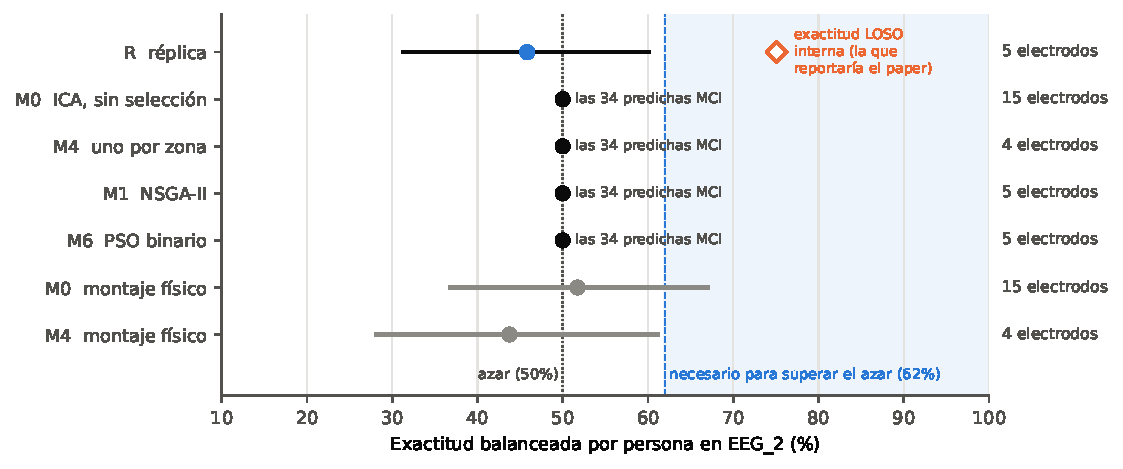
\includegraphics[width=\linewidth]{../figs/es_main.pdf}
\caption{\textbf{Ningún método detectó MCI por encima del azar en personas nuevas.} Exactitud balanceada por persona en EEG\_2 con IC bootstrap del 95\,\%. La zona sombreada es lo que un método necesitaba alcanzar para superar el azar con 34 personas. El rombo es la exactitud LOSO interna de la réplica en EEG\_1, la cifra que reportaría el procedimiento del artículo original. Cuatro métodos predijeron MCI para las 34 personas, por lo que su exactitud es exactamente 50\,\% sin dispersión.}
\label{fig:main}
\end{figure}

\paragraph{PI: ningún método superó el azar.} Tras la corrección de Holm, ningún método superó el azar ($p_\text{Holm}=1.00$ en los cinco). La réplica R clasificó bien a 15 de 34 personas (exactitud balanceada 45.8\,\%), con sensibilidad de 16.7\,\% y especificidad de 75.0\,\%; su exactitud por segmento fue 45.6\,\%. M0, M4, M1 y M6 predijeron MCI para todas las personas de EEG\_2 (sensibilidad 100\,\%, especificidad 0\,\%), un resultado degenerado que se explica en la Sección~\ref{sec:shift}.

\paragraph{H1 se confirmó.} En EEG\_1, NSGA-II eligió T3, Cz, T4, Pz y P4 (dos de ellos, Cz y T4, entre los más elegidos por \citealp{aljalal2024}) con una exactitud LOSO interna de 75.1\,\%, la cifra que reportaría el procedimiento original. Este valor queda por encima del límite superior del IC del 95\,\% de la exactitud balanceada externa (60.1\,\%); la caída fue de 29.3 puntos.

\paragraph{H2 y H3 se cumplieron solo de forma trivial.} M0 resultó formalmente no inferior a R (diferencia $+4.2$ puntos, IC 90\,\% $-7.6$ a $+16.0$, $p=0.026$) y M4 formalmente no inferior a M1 con menos electrodos (4 frente a 5; diferencia 0, $p_\text{Holm}<0.001$). M6 usó la misma mediana de electrodos que M1, así que su parte de H3 no se confirmó. Como M0, M4, M1 y M6 predijeron la misma clase para todas las personas, estas comparaciones no son informativas: muestran que una predicción constante no es peor que R ni que otra predicción constante, no que los métodos más limpios o más parsimoniosos detecten MCI (Fig.~\ref{fig:diff}).

\paragraph{H4 fue no concluyente.} El montaje físico cambió la exactitud balanceada en $+1.7$ puntos para M0 (IC 90\,\% $-10.4$ a $+14.3$; $p_\text{Holm}=0.15$) y en $-6.2$ puntos para M4 ($-20.5$ a $+8.3$; $p_\text{Holm}=0.31$). Ambos intervalos incluyen el margen y el cero, así que no se demostró la no inferioridad ni tampoco la inferioridad.

\begin{figure}[t]
\centering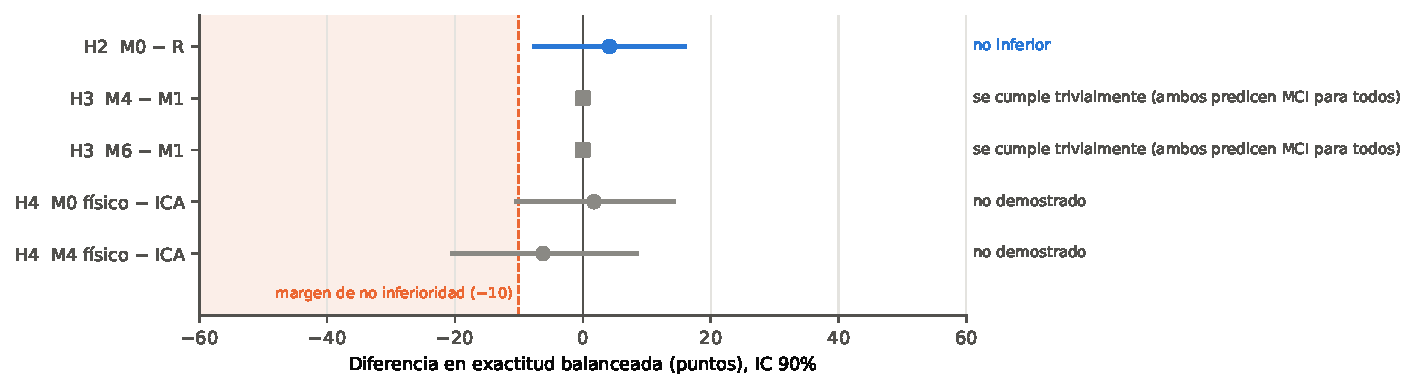
\includegraphics[width=\linewidth]{../figs/es_diff.pdf}
\caption{\textbf{Comparaciones pareadas preregistradas.} Diferencia en exactitud balanceada en las mismas 34 personas con IC bootstrap pareado del 90\,\%; la no inferioridad requería que el límite inferior quedara por encima de $-10$ (línea discontinua). Los cuadrados marcan comparaciones entre dos métodos que predijeron MCI para todos, que se cumplen de forma trivial.}
\label{fig:diff}
\end{figure}

\subsection{Por qué fallaron los métodos: cambio de dominio y confusores de adquisición}\label{sec:shift}

\paragraph{Las dos bases se distinguen casi perfectamente.} El control descriptivo identificó la base de origen de las 58 personas a partir de sus características de 15 electrodos con 94.4\,\% de exactitud balanceada, muy por encima del umbral de 75\,\% que registramos para un cambio de dominio grande. En EEG\_2 la banda delta concentró en promedio el 68.8\,\% de la potencia de 1--30\,Hz, frente a 39.7\,\% en EEG\_1, mientras que alfa bajó de 21.7\,\% a 8.0\,\% (Fig.~\ref{fig:conf}, izquierda). En EEG\_1 el grupo MCI tenía más delta que los controles (43.5\,\% frente a 36.4\,\%), así que todos los modelos aprendieron que más delta significa MCI; al aplicarlos a EEG\_2, donde todos tienen más delta que cualquier persona de EEG\_1, asignaron a las 34 personas a MCI. Dentro de EEG\_2 la dirección se invirtió (67.1\,\% en MCI frente a 70.7\,\% en controles).

\begin{figure}[t]
\centering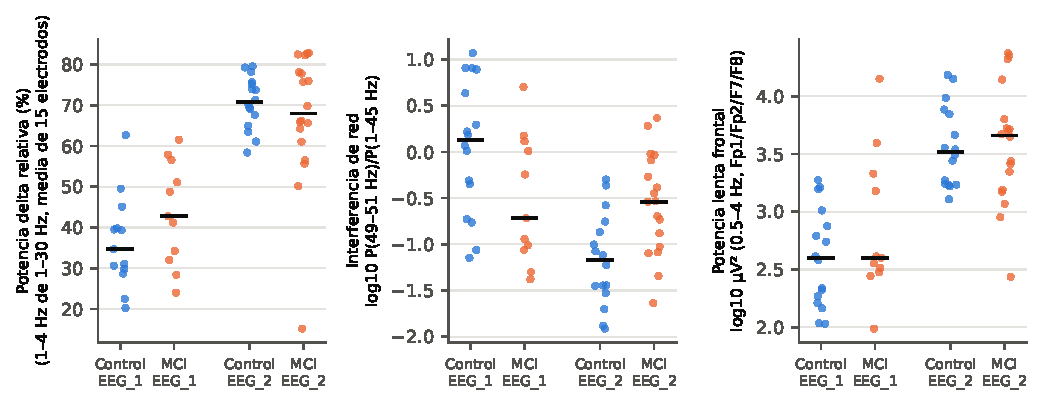
\includegraphics[width=\linewidth]{../figs/es_conf.pdf}
\caption{\textbf{Las diferencias entre bases son mayores que las diferencias entre grupos.} Cada punto es una persona; las barras son medianas. Izquierda: potencia delta relativa, la característica que mueve a los clasificadores. Centro: interferencia de la red eléctrica en los registros originales; su asociación con el diagnóstico se invierte entre bases. Derecha: potencia lenta frontal, unas nueve veces mayor en EEG\_2.}
\label{fig:conf}
\end{figure}

\paragraph{La interferencia de la red se asocia con la etiqueta, en sentidos opuestos.} La potencia relativa en 49--51\,Hz de los registros originales difirió entre bases ($p<0.001$) y se asoció con el diagnóstico en ambas, pero en sentidos opuestos: en EEG\_1 los controles tenían más interferencia que los MCI (AUC 0.28 de la interferencia como predictor de MCI; $p=0.064$), mientras que en EEG\_2 los MCI tenían más interferencia que los controles (AUC 0.79; $p=0.004$). Las condiciones de adquisición están entrelazadas con los grupos diagnósticos de una forma que no se transfiere entre bases.

\paragraph{Los puntajes de los modelos siguen a la actividad lenta frontal.} La potencia lenta frontal (0.5--4\,Hz en Fp1, Fp2, F7 y F8) fue unas nueve veces mayor en EEG\_2 ($p<0.001$) y no difirió entre grupos dentro de ninguna base. En EEG\_2, el puntaje continuo de M0 se correlacionó con esta potencia lenta frontal (Spearman $\rho=0.42$, $p=0.012$) y no significativamente con el diagnóstico (AUC 0.52), aun cuando los electrodos frontales se habían eliminado y los componentes oculares restado.

\subsection{Análisis exploratorios}

\paragraph{Tampoco hay señal de ordenamiento.} El AUC, que no depende del umbral de decisión y por tanto no se ve afectado por un desplazamiento global, fue 0.52 para M0, 0.47 para M4, 0.44 para M0-físico y 0.40 para M4-físico. Entrenar con las 27 personas de EEG\_1 no cambió el panorama (AUC 0.41--0.54). En un análisis \emph{post hoc} no preregistrado, estandarizar cada base con su propia media y desviación estándar (sin etiquetas) eliminó el desplazamiento global pero no reveló señal: AUC 0.52 para M0 ($p=0.44$) y 0.45 para M4 con ICA, 0.42 y 0.38 con el montaje físico.

\paragraph{El control positivo apuntó en la dirección esperada, pero fue débil.} La potencia alfa relativa posterior fue menor en MCI que en controles en ambas bases, como se esperaba \citep{babiloni2015}, pero el efecto fue pequeño y no significativo (AUC 0.59, $p=0.49$ en EEG\_1; 0.57, $p=0.48$ en EEG\_2; similar con el montaje físico).

\paragraph{Los electrodos elegidos fueron estables pero no válidos.} M1 eligió el mismo subconjunto (F4, T4, T5, Pz, T6) con cuatro de cinco semillas, y M6 eligió T4 y T6 con las cinco semillas y F4 y Pz con cuatro (Fig.~\ref{fig:heads}). Esta estabilidad entre semillas no se tradujo en desempeño externo.

\begin{figure}[t]
\centering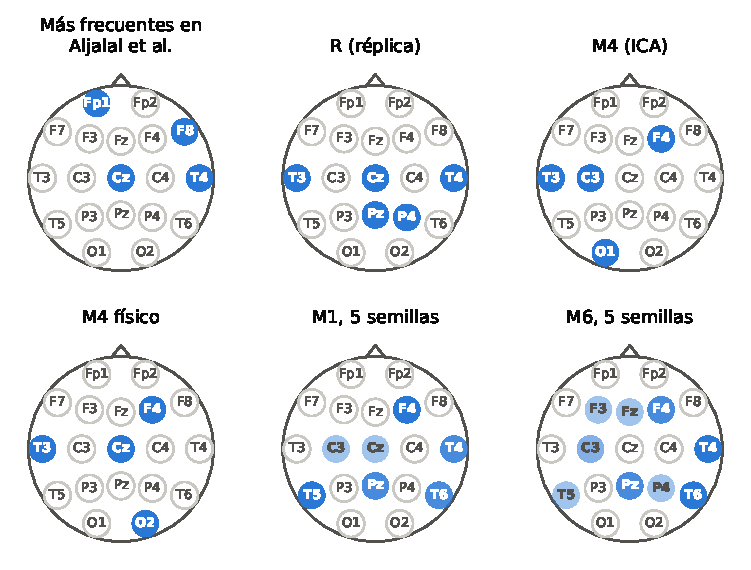
\includegraphics[width=0.82\linewidth]{../figs/es_heads.pdf}
\caption{\textbf{Electrodos elegidos en EEG\_1.} Más oscuro significa elegido con más frecuencia (entre semillas en M1 y M6). Fp1 y F8, dos de los electrodos más elegidos por \citet{aljalal2024}, están entre los más contaminados por movimientos oculares; M0--M6 excluyen Fp1, Fp2, F7 y F8 por diseño.}
\label{fig:heads}
\end{figure}

\section{Discusión}

En una prueba externa preregistrada, una réplica independiente de la selección de electrodos con NSGA-II para detectar MCI alcanzó 75.1\,\% de exactitud interna con cinco electrodos y 45.8\,\% de exactitud balanceada en 34 personas que nunca había visto. Cuatro alternativas construidas para evitar los problemas conocidos no lo hicieron mejor: todas clasificaron a cada persona nueva como MCI. Ningún método, con ningún número de electrodos ni con ninguno de los dos montajes, detectó MCI por encima del azar en la cohorte nueva.

\paragraph{De dónde vienen las exactitudes publicadas.} Tres mecanismos, cada uno medido en los datos de desarrollo, pueden explicar la diferencia entre las exactitudes publicadas y nuestros resultados. Primero, cuando segmentos de la misma persona se usan para entrenar y probar, se alcanzan exactitudes de 90--99\,\% con características que dan resultados al nivel del azar cuando las personas se mantienen separadas; la cifra con todos los canales reportada por \citet{aljalal2024} está más cerca de lo primero. Con el artículo no podemos saber cómo se construyeron los pliegues, así que esta es una afirmación de compatibilidad, no sobre su código. Segundo, NSGA-II alcanza 72--79\,\% de exactitud interna con etiquetas revueltas, así que una exactitud interna de 75\,\% después de la selección no aporta evidencia de valor diagnóstico; la evaluación anidada y la prueba externa eliminan este sesgo \citep{varma2006,cawley2010}. Tercero, dos de los electrodos elegidos con más frecuencia (Fp1 y F8) están dominados por señal ocular. Estos mecanismos no requieren ningún error en el análisis original: son el comportamiento esperado de una búsqueda sin restricciones evaluada en las mismas 24 personas, y por eso los atendimos por diseño y probando en personas nuevas.

\paragraph{El cambio de dominio domina.} El hallazgo más informativo no estaba planteado como hipótesis: dos bases públicas del mismo centro y sistema de registro se distinguen en 94\,\% solo por su EEG, y la diferencia (un espectro dominado por delta en EEG\_2, nueve veces más potencia lenta frontal y un perfil distinto de interferencia de red) es mayor que cualquier diferencia entre MCI y controles. Con los archivos publicados no podemos determinar su causa; la vigilancia, la impedancia de los electrodos, el filtrado o el periodo de registro son explicaciones posibles. Su consecuencia, en cambio, es clara: un modelo que aprendió una pequeña diferencia de potencia delta entre grupos moverá a toda la cohorte nueva al otro lado de su frontera de decisión. La estandarización por base eliminó el desplazamiento global pero no reveló señal residual, así que el fallo no es solo un problema de calibración. La asociación opuesta entre la interferencia de red y el diagnóstico en las dos bases muestra que las condiciones de adquisición pueden confundirse con los grupos. En bases tan pequeñas, cualquier método que busque ampliamente, ya sea que optimice electrodos, características o clasificadores, probablemente encontrará estos confusores.

\paragraph{Qué lograron y qué no las alternativas más limpias.} Las alternativas se diseñaron para eliminar tres fuentes de optimismo: la fuga entre segmentos, el sesgo de selección y la contaminación ocular. Lo lograron en el sentido de que sus estimaciones internas fueron honestas (alrededor de 61--64\,\% en LOSO anidado, nunca por encima del azar), pero no crearon una señal que no existe en estos datos. Las confirmaciones formales de H2 y H3 no son evidencia de que funcionen; solo muestran que su fallo no fue peor que el del método original. La selección parsimoniosa al menos no perjudicó, y los electrodos que eligieron NSGA-II y PSO fueron estables entre semillas. Sin embargo, la estabilidad no implicó validez: un subconjunto estable puede estar ajustado de forma estable a un confusor.

\paragraph{Electrodos virtuales frente a físicos.} Los estudios de minimización de electrodos suelen calcular cada canal después de una referencia promedio y una ICA sobre el montaje completo, y luego reportan los canales elegidos como si un dispositivo pudiera usarlos solos. El montaje físico pone esto a prueba directamente. En desarrollo, el método de un electrodo por zona perdió la mayor parte de su exactitud con electrodos físicos; en la prueba externa la comparación fue no concluyente porque ninguno de los dos montajes funcionó. Recomendamos que los estudios futuros reporten ambas versiones.

\paragraph{Recomendaciones.} A partir de estos resultados proponemos el siguiente protocolo mínimo para estudios que eligen electrodos de EEG con fines diagnósticos: evaluar por persona, nunca por segmento; mantener la selección dentro del ciclo de validación (anidada); comparar contra el mismo procedimiento corrido con etiquetas revueltas; reportar el AUC además de la exactitud; revisar si los electrodos elegidos están contaminados por movimientos oculares y si variables de adquisición (como la interferencia de red) difieren entre grupos; reportar una versión con montaje físico; probar si las bases se pueden distinguir antes de combinarlas o transferir modelos entre ellas; y preregistrar una prueba externa única \citep{nosek2018,collins2024}.

\paragraph{Limitaciones.} Los tamaños de muestra son pequeños, así que la prueba externa solo podía detectar efectos grandes (potencia de 0.84 para una exactitud balanceada real de 70\,\%) y las hipótesis no confirmadas son no concluyentes más que negativas. EEG\_2 se publicó como extensión de la misma base, pero no pudimos verificar que sus criterios diagnósticos y de inclusión, su protocolo de registro o su periodo sean idénticos, y la causa del cambio de dominio sigue sin conocerse. Nuestra réplica descansa en supuestos documentados donde el artículo original no es específico (familia wavelet, umbral de entropía, operadores genéticos, qué controles se excluyeron), y la prueba externa cubrió la mejor configuración de selección de canales del artículo (DWT, ThEn, análisis discriminante), no todas las combinaciones de características ni la selección conjunta de características de su Experimento III. Solo se analizaron los primeros 10 minutos de cada registro, no había información de edad ni sexo y la regla de componentes de ICA fue automática. Algunos diagnósticos de desarrollo (etiquetas revueltas, contaminación ocular) se calcularon antes del registro y se reportan como resultados de desarrollo. Por último, la estandarización por base fue \emph{post hoc}. Ninguna de estas limitaciones favorece la conclusión de que las exactitudes originales se transfieren: si acaso, cada una facilitaría encontrar una señal transferible.

\section{Conclusiones}

Las altas exactitudes reportadas para la selección de electrodos con NSGA-II en la detección de MCI con EEG en reposo no sobrevivieron a una prueba externa independiente y preregistrada: una exactitud interna de 75\,\% se convirtió en 46\,\% en personas nuevas, y ninguna de cuatro alternativas más limpias o más parsimoniosas superó el azar. El factor decisivo fue un gran cambio de dominio entre dos bases del mismo centro, junto con variables de adquisición asociadas a los grupos diagnósticos. Minimizar electrodos solo tiene sentido una vez que se demostró que una señal generaliza; hasta entonces, recomendamos una evaluación por persona, anidada y validada externamente, con montajes físicos y análisis preregistrados.
